\chapter{Electrones en un potencial periódico: teoría de bandas} \label{Ch:07}

Para mejorar algunas de las predicciones del modelo de gas de electrones libres se introduce la interacción de los electrones con la red cristalina a través de un potencial periódico, despreciando las interacciones entre electrones. En este tema vamos a usar los temas 11 y 15 del Oxford Solid State \cite{Oxford_Solid_State}, en vez del tema 7 de \cite{Fisica_del_Estado_Solido}, ya que consideramos que, como muchos temas, está todo muy mal redactado.

\section{Cadena de electrones}

En los capítulos anteriores hemos considerado las propiedades de los fonones a través de un sistema unidimensional y luego lo hemos generalizado para varias dimensiones. En este punto vamos a hacer un tratamiento similar de los electrones, considerando ondas de electrones en vez de fonones (cabe destacar que en la mecánica cuántica y en la teoría cuantica de campos los electrones son ondas, por lo que en realidad esta asunción no está tan alejada de la realidad).

\subsection{Cadena de electrones en una dimensión}

Para tratar de describir un sistema de electrones en un átomo/molécula usamos la teoría LCAO\footnote{De sus siglas en inglés \textit{Linear Combination of Atomic Orbitales}, en español \textit{Combinación Lineal de Orbitales Atómicos} o CLOA}, que nos dice que podremos suponer que los orbitales moleculares son un conjunto de combinaciones lineales de orbitales atómicos (denotados por $n,l,m_l,m_s$). En esta imagen asumimos que solo tenemos un orbital en el átomo $n$ y lo denotamos por $|n \rangle$. Por conveniencia y facilidad aplicamos condiciones de contorno de tal manera que si hay $N$ sitios, el sitio $N$ y $0$ es el mismo. Además consideremos qeu los orbitales son ortogonales entre sí:

\begin{equation}
	\langle n | m \rangle = \delta_{n,m}
\end{equation}
Supongamos ahora la función más general del sistema, dada por una combinación de las diferentes funciones orbitales:

\begin{equation}
	|\Psi \rangle = \sum_n \phi_n |n\rangle
\end{equation}
Si la función de ondas es solución de la ecuación de Schödinger tenemos que:

\begin{equation}
	\Hcal |\Psi \rangle = E |\Psi \rangle
\end{equation}
tal que:

\begin{equation}
	\sum_m \Hcal \phi_m |m\rangle =  \sum_m E \phi_m |m\rangle
\end{equation}
Si ahora aplicamos $\langle n |$, como $\langle n| \Hcal | m \rangle= H_{mn}$ no es necesariamente cero, tenemos que el problema los autovalores se ha convertido en un conjunto de ecuaciones lineales (conocidos los valores $H_{nm}$) tal que:


\begin{equation}
	\sum_m H_{mn} \phi_m  =  E \phi_n
\end{equation}
De tal manera que la solución mas general no es más que una combinación lineal de las soluciones orbitales que calculemos con el modelo. En realidad esta solución es una aproximación, llamada \textit{método variacional}, y será mejor cuantos más orbitales pongamos en el modelo. Si en vez de tener un solo orbital $|n\rangle$ por sitio, tuviéramos varios $|n,\alpha\rangle$ siendo $\alpha$ un conjunto de números, tendríamos cuanto mas amplio el conjunto una solución cada vez más cerca de la real.

Este método es el llamado LCAO pero aplicado para nuestra cadena de electrones. Sin embargo esto trae el problema de que la condición de ortogonalidad ya no se verifica $\langle n ,\alpha | m,\beta \rangle \neq \delta_{nm} \delta_{\alpha \beta}$. En general asumiremos, de existir un solo orbital por sitio, que la ortogonalidad se verifica. Nuestro hamiltoniano vendrá dado por:

\begin{equation}
	\Hcal = \Hcal_0 + \sum_{j} V_j
\end{equation}
siendo $\Hcal_0 = \pn^2 /2m$ la energía cinética y $V_j$ la interacción de Coulomb en del electrón en la posición $\rn$ en el núcleo ubicado en $j$:

\begin{equation}
	V_j = V(\rn-\Rn_j)
\end{equation}
Con estas definiciones tenemos que la solución:

\begin{equation}
	\Hcal |m\rangle = (\Hcal_0 + V_m) |m\rangle + \sum_{j\neq m} V_j |m\rangle
\end{equation}
Lógicamente $\Hcal_0 +V_m |m\rangle = \varepsilon_{at}|m\rangle$ (siendo $\varepsilon_{at}$ la energía atómica). Así tenemos que:

\begin{equation}
	H_{nm} = \langle n | \Hcal | m \rangle = \varepsilon_{at} \delta_{nm}+\sum_{j\neq m} \langle n |V_j |m\rangle
\end{equation}
Si suponemos que la interacción $\langle n | V_j | m \rangle$ solo ocurre entre los primeros vecinos, tal que:

\begin{equation}
	\sum_{j\neq m} \langle n |V_j |m\rangle = \left\lbrace \begin{array}{lc}
		V_0 & \ n=m \\
		-t & \ n=m\pm 1 \\
		 0 & \text{cualquier otro n}
	\end{array} \right.
\end{equation}
Nótese que la matriz $H$ no está diagonalizada, ya que los términos $n\neq m$ no son nulos, con un valor (si $\varepsilon_0 = \varepsilon_{at}+V_0$)

\begin{equation}
	H_{nm} = \varepsilon_0 \delta_{nm} - t(\delta_{n,n+1}+\delta_{n,n-1})
\end{equation}

\subsection{Solución a la cadena de electrones unidimensional}

La solución a a la cadena de electrones monoatómica es bien sencilla: es una combinación de ondas planas. Supongamos entones que la solución es

\begin{equation}
	\phi_n = \frac{e^{ikna}}{\sqrt{N}}
\end{equation}
donde el $1/\sqrt{N}$ es el factor de normalización. Sustituyendo esto en la ecuación de Schrödinger independiente del tiempo (si quisiéramos resolver la ec. dependiente del tiempo solo tendríamos que añadir un término $e^{i\omega t}$). Podemos ver en nuestra solución que $k\rightarrow k + 2 \pi /a$ también es una solución. Además si aplicamos las condiciones de contorno obtenemos que nuestros momentos se cuantizan en unidades de $2\pi /L$. 

En cualquier caso, sustituyendo la solución de ondas planas en nuestra ecuación tenemos que:

\begin{equation}
	\sum_m H_{nm} \phi_m = \varepsilon_0 \frac{e^{-ikna}}{\sqrt{N}} - t \parentesis{\frac{e^{-ik(n+1)a}}{\sqrt{N}}+\frac{e^{-ik(n-1)a}}{\sqrt{N}}} = E \frac{e^{-ikna}}{\sqrt{N}} = E\phi_n
\end{equation}
de lo que obtenemos el espectro de energías:

\begin{equation}
	E=\varepsilon_0 - 2 t \cos (ka)
\end{equation}
que se parece bastante al espectro de nuestro fonón unidimensional. La curva de dispersión, periódica en $k\rightarrow k+2\pi/a$, tiene una región donde la velocidad de grupo es cero en $k=n\pi/a$ para cualquier $n$ entero. A diferencia de los electrones libres, la ecuación de dispersión de los electrones nos da un valor máximo y mínimo de la energía, ahora está acotada. Consecuentemente los electrones solo tienen autvalores en una determinada \textbf{banda} de energías. El término banda se usa entonces para describir el rango posible de valores energéticos en el cual se puede encontrar el electrón y para describir una rama conectada para una función de dispersión (en esta imagen solo hay un modo posible para cada $k$, pero en general tendremos más).

La diferencia energética entre el máximo y mínimo de la banda se le llama \textit{ancho de banda}. Estados con energías mas allá del ancho de banda (o con menos energías) no son posibles. El ancho de banda lo determina el término $t$ o ``término de hopping'', que depende, de varios términos, como la distancia entre átomos. El término $t$ nos da un valor de la energía de intercambio, es decir, la energía que cuesta transferir el electrón del átomo $m$ al $m\pm 1$. Para pequeños $k$ tenemos que la ecuación de dispersión nos queda como

\begin{equation}
	E(k) = \cte + ta^2 k^2
\end{equation}
El resultado del comportamiento parabólico es muy similar al de los electrones libres, por lo que si relacionamos ambos términos de dispersión salvo que ahora $m\rightarrow m^* $:

\begin{equation}
	\frac{\hbar^2 k^2}{2m^* } = t a^2 k^2
\end{equation}
tal que

\begin{equation}
	m^* = \parentesis{\hbar^2}{2ta^2}
\end{equation}
es la \textbf{masa efectiva}, que se define como aquella masa la cual debería tener el electrón para que a bajos $k$ la dispersión se comporte como un conjunto de masa $m^*$. Evidentemente la masa efectiva no tiene ninguna relación con la masa del electrón, pero si con el término de intercambio. 

\subsection{Introducción al llenado de bandas}

Imaginemos ahora que nuestra cadena lineal de electrones está realmente de átomos que ``donan'' un electrón a la banda. Dado que tenemos $N$ estados $k$ posibles (recordemos que hemos impuesto que la cadena lineal cumple condiciones de contorno periódicas) en la banda, es de suponer que, como los electrones son fermiones, la banda se llenará. Sin embargo hay 2 estados de espín, por lo que en realidad la banda esta medio llena. Evidentemente si aplicamos un campo eléctrico pequeño, se desplazan los estados ocupados hacia la derecha de tal modo que aparece un momento total no cero, y por tanto aparece una corriente. Esto explica porqué muchos cristales de átomos monovalentes son metales.

Por otro lado, si cada átomo de nuestro momento fuera divalente (dona 2 electrones a la banda) tendremos que la banda estaría llena: no existe campo eléctrico que pueda mover $k$ hacia un lado u otro, ya que todos los estados posibles de $k$ están ocupados. Es decir, \textit{las bandas ocupadas no pueden llevar corriente}.


\subsection{Múltiples bandas}

En el modelo introducido, hemos considerado que solo hay un átomo en la celda unidad y un sólo orbital por átomo. Lógicamente para mejorar el modelo deberíamos considerar que hay mas de un orbital por cada átomo/celda unidad. Una posibilidad es considerar más de un electrón por átomo pero celdas monoatómicas. 

Otra es considerar que hay un orbital posible pero varios átomos por celda unidad. Por ejemplo si tenemos dos átomos por celda, existirán dos bandas posibles, análogo a lo que pasaba a la cadena diatómica de átomos, teniendo dos posibles valores de la energía para cada $k$. En el lenguaje de los fonones hablabamos de ramas acústicas y ramas ópticas, en el caso de los electrones decimos simplemente que hay dos bandas.

\begin{Anotacion}
	\textcolor{red}{Hay que añadir mas cosas que mencionaba nuestro libro del Oxford}
\end{Anotacion}	

\section{Aproximación de red vacía}

En la sección anterior hemos descrito algunas de las propiedades de los electrones en un potencial periódico para el modelo unidimensional. Ahora haremos la expansión a 3 dimensiones y a un potencial muy débil. De hecho la sección anterior es el caso opuesto al que vamos a estudiar aquí, ya que suponía electrones muy fuertemente ligados a los átomos. Supongamos que nuestro hamiltoniano viene dado por:

\begin{equation}
	\Hcal = \Hcal_0 + V(\rn)
\end{equation}
tal que $V(\rn)$ es periódico, es decir que verifica 

\begin{equation}
	V(\rn+\Rn)=V(\rn)
\end{equation}
donde $\Rn$ es un \textbf{vector de red}. Como sabemos los autoestados de la ecuación de Schrödinger libre (sin potencial) son ondas planas denotadas por $|\kn\rangle$ tal que

\begin{equation}
	|\kn\rangle \equiv A e^{i\kn \rn}
\end{equation}
donde la energía viene dada por

\begin{equation}
	\varepsilon_0 = \frac{\hbar^2 |\kn|^2}{2m}
\end{equation}
El valor medio $\langle \kn'|V|\kn \rangle$ debe venir dado por:


\begin{equation}
	\langle \kn'|V|\kn \rangle  = \frac{1}{L^3} \int \D \rn e^{i(\kn-\kn')\cdot \rn} V(\rn) \equiv V_{\kn'-\kn}
\end{equation}
que es cero a no ser que $\kn'-\kn$ sea un \textit{vector de la red recíproca}. Consecuentemente cualquier solo ondas planas separadas por un vector de red recíproca $\Gn$ pueden interactuar. Aplicando teoría de perturbaciones tenemos que:

\begin{equation}
	\varepsilon(\kn)  =\varepsilon_0 (\kn) + \langle \kn |V|\kn \rangle = \varepsilon_0 (\kn) + V_0
\end{equation}
nos mueve un término $V_0$ todos los posibles autovalores (siendo este su único efecto). Lógicamente este término no va a afectar nada a la física de nuestro problema, por lo que asumir que es cero solo simplifica las ecuaciones. La teoría de perturbaciones de segundo orden nos dice que


\begin{equation}
	\varepsilon(\kn)  =\varepsilon_0 (\kn) + \sum_{\kn'=\kn+\Gn} \frac{\langle \kn' |V|\kn \rangle}{  \varepsilon_0 (\kn) - \varepsilon_0 (\kn')}
\end{equation}
donde el $'$ nos dice que $\Gn \neq 0$. Entonces existen 3 posibilidades:

\begin{itemize}
	\item Que $\varepsilon(\kn')\neq \varepsilon(\kn)$. En ese caso tenemos que $\varepsilon(\kn) \approx \varepsilon_0(\kn)$, ya que estamos suponiendo que el potencial periódico es muy débil y por  tanto $\langle \kn' |V|\kn \rangle \ll \varepsilon(\kn) - \varepsilon(\kn')$. 
	\item Que se verifique que $\varepsilon(\kn')=\varepsilon(\kn)$, es decir que el estado con dicha energía está \textit{degenerado}. Debido a que $\varepsilon(\kn')=\varepsilon(\kn)$ y que $\kn'=\kn+\Gn$ con $\Gn\neq 0$, tenemos que la única posibilidad es que 
	\begin{equation}
		k'=-k = \frac{n\pi}{a}
	\end{equation}
	donde $a$ es la distancia característica de la red.	Es decir, los únicos estados degenerados de energía son aquellos que están en las zonas de frontera de Brillouin.
	\item Que se verifique que $\varepsilon(\kn')\approx\varepsilon(\kn)$, es decir que el estado con dicha energía está casi degenerado. Debido a que $\varepsilon(\kn')\approx\varepsilon(\kn)$, cosa que solo pasa si la diferencia entre ambos es $\Gn$ y el vector de onda está muy próximo del plano de Bragg, tal que $k\approx n\pi/a$, tendremos que $\langle \kn' |V|\kn \rangle \sim \varepsilon(\kn) - \varepsilon(\kn')$ y por tanto no es despreciable.
	
\end{itemize}	

Como podemos ver esto nos lleva a que los vectores de onda que no estén en una de la zonas de frontera de Brilluoin (es decir, que caigan en un plano de Braggs) tienen una energía $\varepsilon(\kn)$, y por tanto cuanto mas lejos del plano de Bragg más válido será el comportamiento de electrones libres.

\subsection{Teoría de perturbaciones para estados degenerados}

Para estados degenerados la teoría de perturbaciones nos dice que los autoestados son una combinación lineal de los estados originales, y los autovalores una combinación de ambos también. Entones el problema es básicamente diagonalizar $\Hcal$, para lo cual tenemos que conocer los términos de la matriz, dados por:

\begin{eqnarray*}
	\langle \kn | \Hcal |\kn \rangle &= & \varepsilon_0(\kn) \\	
	\langle \kn' | \Hcal |\kn \rangle' &= & \varepsilon_0(\kn')=\varepsilon(\kn+\Gn) \\	
	\langle \kn' | \Hcal |\kn \rangle &= & V_{\kn-\kn'}=V_{\Gn}^* \\	
	\langle \kn | \Hcal' |\kn \rangle &= & V_{\kn'-\kn}=V_{\Gn}
\end{eqnarray*}
de tal modo que 
\begin{equation}
	\Hcal \equiv \begin{pmatrix}
		\varepsilon(\kn) & V_{\Gn}^* \\ 
		V_{\Gn} & \varepsilon(\kn+\Gn)
	\end{pmatrix}
\end{equation}
Usando el principio variacional, el autoestado será una combinación de $|\kn\rangle$ y $|\kn'\rangle$ que verifique:

\begin{equation}
|\Psi \rangle = \alpha |\kn \rangle + \beta |\kn'\rangle = \alpha |\kn \rangle + \beta |\kn+\Gn\rangle 
\end{equation}
tal que:

\begin{equation}\begin{pmatrix}
	\varepsilon(\kn) & V_{\Gn}^* \\ 
	V_{\Gn} & \varepsilon(\kn+\Gn)
\end{pmatrix} \begin{pmatrix}
	\alpha \\ \beta
\end{pmatrix} = \begin{pmatrix}
	\alpha \\ \beta
\end{pmatrix} 
\end{equation}
Sea $\varepsilon$ el autovalor de $\Hcal$, tenemos que la ecuación para calcularlo es:

\begin{equation}
	\parentesis{\varepsilon_0(\kn)-\varepsilon}\parentesis{\varepsilon(\kn+\Gn)-\varepsilon} - |V_{\Gn}|^2 = 0
\end{equation}
Entonces en función de cada caso tendremos diferentes comportamientos. Veamos cada caso por separado. C

\subsubsection{Vector de ondas en el plano de Bragg}

El caso más simple es en el que precisamente $\kn$ es un vector que cae en el plano de Bragg. En este caso la ecuación se convierte:

\begin{equation}
	\parentesis{\varepsilon_0 (\kn)-E}^2 =|V_\Gn|^2
\end{equation}
Con las dos soluciones:

\begin{equation}
	E_\pm = \varepsilon_0 (\kn) \pm |V_\Gn|
\end{equation}
Es decir, existe un gap en los bordes de la zona de Brillouin (planos de Bragg). Siempre que existan dos momentos $\kn$ y $\kn'$ con una $\varepsilon_0(\kn)$ en presencia de un potencial $V_\Gn$ periódico, los autoestados de energía estarán separados por $\pm |V_\Gn|$.

Es decir, habrá regiones de energía inaccesibles para cualquier estado $|\kn\rangle$, formando, al igual que en la sección anterior, bandas de energía permitidas y bandas de energías prohibidas. Las bandas de energías prohibidas estarán asociadas a los valores $\varepsilon(\kn)$ si $\kn \in $\{PZB,SZB,TZB...\}, tal que la banda es $E\in (\varepsilon(\kn)-V_\Gn,\varepsilon(\kn)+V_\Gn)$. 

\subsubsection{Caso unidimensional}

Para entender el mejor estos conceptos vamos a estudiar el caso unidimensional con un potencial concreto: $V(x)=V_0 \cos (2\pi x/a)$ con $V_0>0$. La frontera de la primera zona de Brillouin (en 1D son puntos, al igual que en 2D son lineas y en 3D planos) son $k=\pi/a$ y $k'=-k=-\pi/a$; de tal modo que se verifica que $k'-k=G$ y que $\varepsilon_0 (k')= \varepsilon_0(k)$. Las soluciones:  

\begin{equation}
	|\psi_\pm \rangle = \frac{1}{\sqrt{2}} \parentesis{|k\rangle \pm |k'\rangle}
\end{equation}
asignando a cada uno de estos los autovalores de energías $E_\pm$ respectivamente. Dado que podemos escribir estas autofunciones como exponenciales complejas, tenemos que:

\begin{equation*}
	\psi_+ \sim e^{ikx/a}+e^{-ikx/a} \propto \cos (x\pi/a)
\end{equation*} 
\begin{equation*}
	\psi_- \sim e^{ikx/a}-e^{-ikx/a} \propto \sin (x\pi/a)
\end{equation*} 
Si nos fijamos en las densidades de probabilidad $|\psi_\pm|^2$ tenemos que la densidad de $\psi_+$ es máxima cuando el potencial $V$ es máximo mientras que $\psi_-$ es máximo cuando el potencial es mínimo, tal y como podemos ver en la figura \ref{Fig:07-01}. Consecuentemente el principio general es que el potencial periódico hace que interfieran las ondas $|\kn\rangle $ y $|\kn+\Gn\rangle$, y cuando estas energías son las mismas, la mezcla de entre ellas es fuerte y ambas se combinan para generar dos estados, una de máxima energía y otra de mínima energía. 


\begin{figure}[h!] \centering
	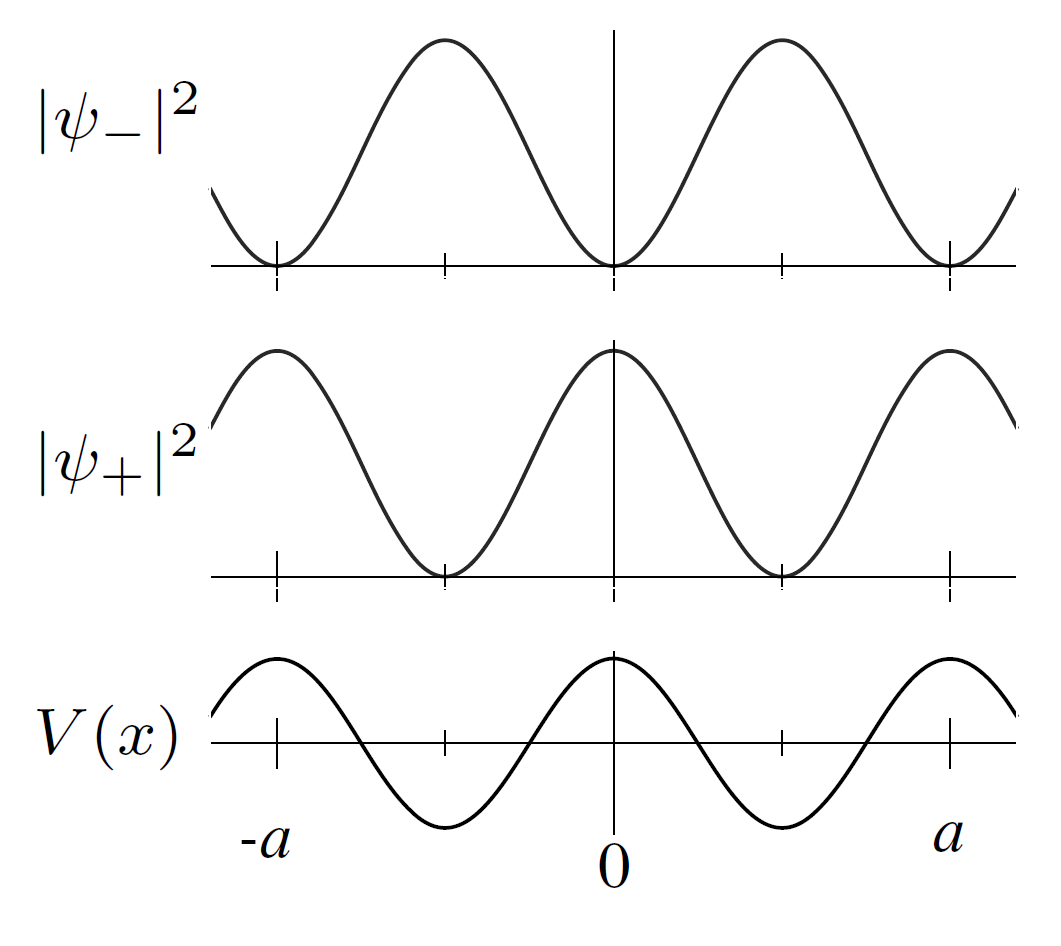
\includegraphics[scale=0.35]{Cuerpo/Ch_07/Oxford-01.png}
	\caption{Forma de las funciones de onda cuando $k=n\pi k/a$.}
	\label{Fig:07-01}
\end{figure}    

\subsubsection{Vector de ondas cerca del plano de Bragg}

No es muy complicado de extender este razonamiento a puntos muy cerca del $\kn$ que esté en la zona de frontera cerca del $\kn$ degenerado. Por simplicidad, seguiremos considerando el caso unidimensional. Supongamos entonces las energías en los estados $k=n\pi/a+\delta$ y $k=-n\pi/a+\delta$. En este caso estamos estudiando vectores de onda en la proximidad del plano de Bragg, tal que

\begin{eqnarray}
	\varepsilon_0 (n\pi/a + \delta) & = & \frac{\hbar^2}{2m} \ccorchetes{\parentesis{n\pi/a}^2 + 2 n \pi \delta / a + \delta^2} \\
	\varepsilon_0 (-n\pi/a + \delta) & = & \frac{\hbar^2}{2m} \ccorchetes{\parentesis{n\pi/a}^2 - 2 n \pi \delta / a + \delta^2}
\end{eqnarray}	
Como podemos ver ahora la ecuación característica (aquella que nos calcula los autovalores de la energía) vendrá dada por:

\begin{equation}
	\parentesis{\frac{\hbar^2}{2m} \ccorchetes{(n\pi/a)}^2 - E + \frac{\hbar^2}{2m} 2 n \pi \delta / a } \parentesis{\frac{\hbar^2}{2m} \ccorchetes{(n\pi/a)}^2 - E - \frac{\hbar^2}{2m} 2 n \pi \delta / a } - |V_{\Gn}|^2 = 0
\end{equation}
que despejando:

\begin{equation}
	\parentesis{\frac{\hbar^2}{2m} \ccorchetes{(n\pi/a)}^2 - E }^2 = \parentesis{ \frac{\hbar^2}{2m} 2 n \pi \delta / a }^2+|V_{\Gn}|^2 
\end{equation}
de tal modo que la solución viene dada por: 

\begin{equation}
	E_\pm = \frac{\hbar^2}{2m} \ccorchetes{(n\pi/a)^2+\delta^2} \pm \sqrt{\parentesis{ \frac{\hbar^2}{2m} 2 n \pi \delta / a }^2+|V_{\Gn}|^2 }
\end{equation}
y si $\delta \ll 1$

\begin{equation}
	E_\pm = \frac{\hbar^2(n\pi/a)^2}{2m} \pm |V_G| + \frac{\hbar^2 \delta^2}{2m}\ccorchetes{1\pm \frac{\hbar^2 (n\pi/a)^2}{m} \frac{1}{|V_G|}}
\end{equation}
Como podemos ver cerca de la zona de Brilluoin el valor de $E_\pm$ depende de $\delta^2$, lo  que significa que cerca de las bandas prohibidas tenemos espectros parabólidos, como vemos en la imagen \ref{Fig:07-02}. Esto se parece mucho a la estructura de la primera sección, de tal forma que aparecen bandas energéticas donda existen autoestados válidos, llamadas \textbf{bandas permitidas}, y las bandas donde hay gaps de energía y no hay estados posibles para dichas energías, formado las \textbf{bandas prohibidas}.

\begin{figure}[h!] \centering
	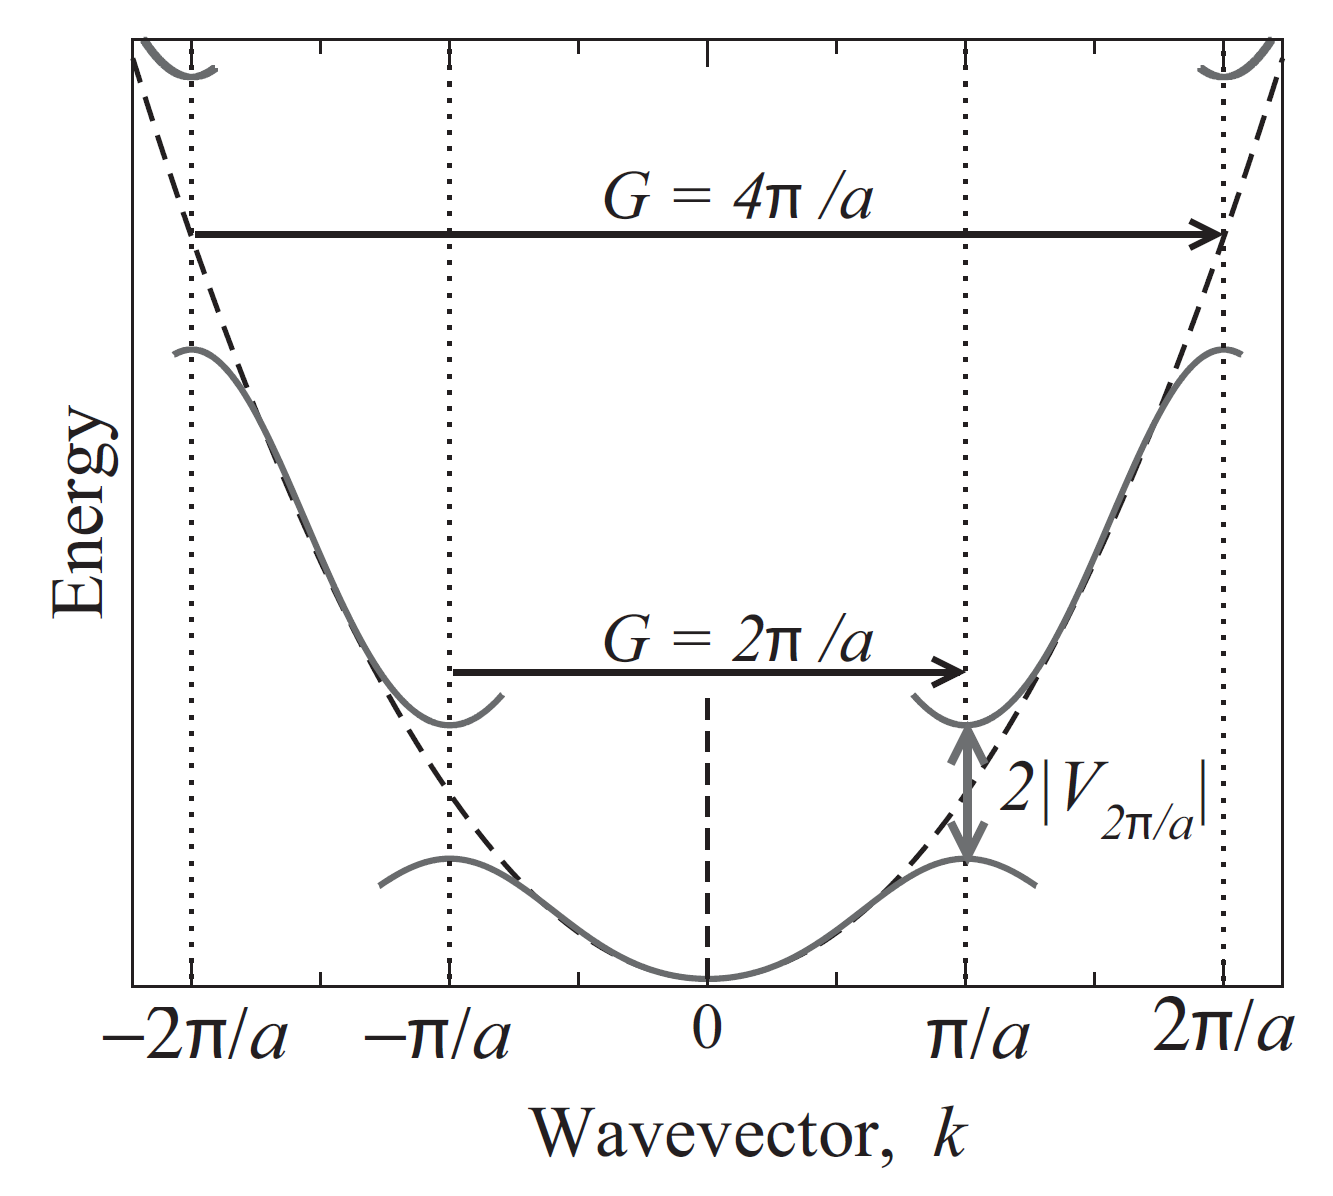
\includegraphics[scale=0.45]{Cuerpo/Ch_07/Oxford-02.png}
	\caption{Dispersión del momento en la región de casi electrones libres, pudiéndose observar que los momentos cerca de la zona de Brilluoin se comportan como parábolas.}
	\label{Fig:07-02}
\end{figure}    
	
En la siguiente imagen podemos ver cual es la forma de la dispersión de energía en dos esquemas que tenemos que tener muy claro que aportan la misma información, solo que uno lo hace de una manera mucho más compacta. Aunque pueda parecer que la zona reducida (\ref{Fig:07-03b}) nos dice que para cada $k$ tenemos varios valores posibles de energía, eso no es verdad. Cuando pasamos de una línea inferior a una línea superior estamos sumando al $\kn$ un $\Gn$, en el caso 1D estamos sumando a $k$ un valor $\pi/a$, obteniendo así las diferentes líneas. Nosotros recomendamos trabajar con el esquema extendido, ya que nos proporciona la misma información pero sin ningún tipo de confusión.

\begin{figure}[h!] \centering
\begin{subfigure}{0.45\linewidth} \centering 
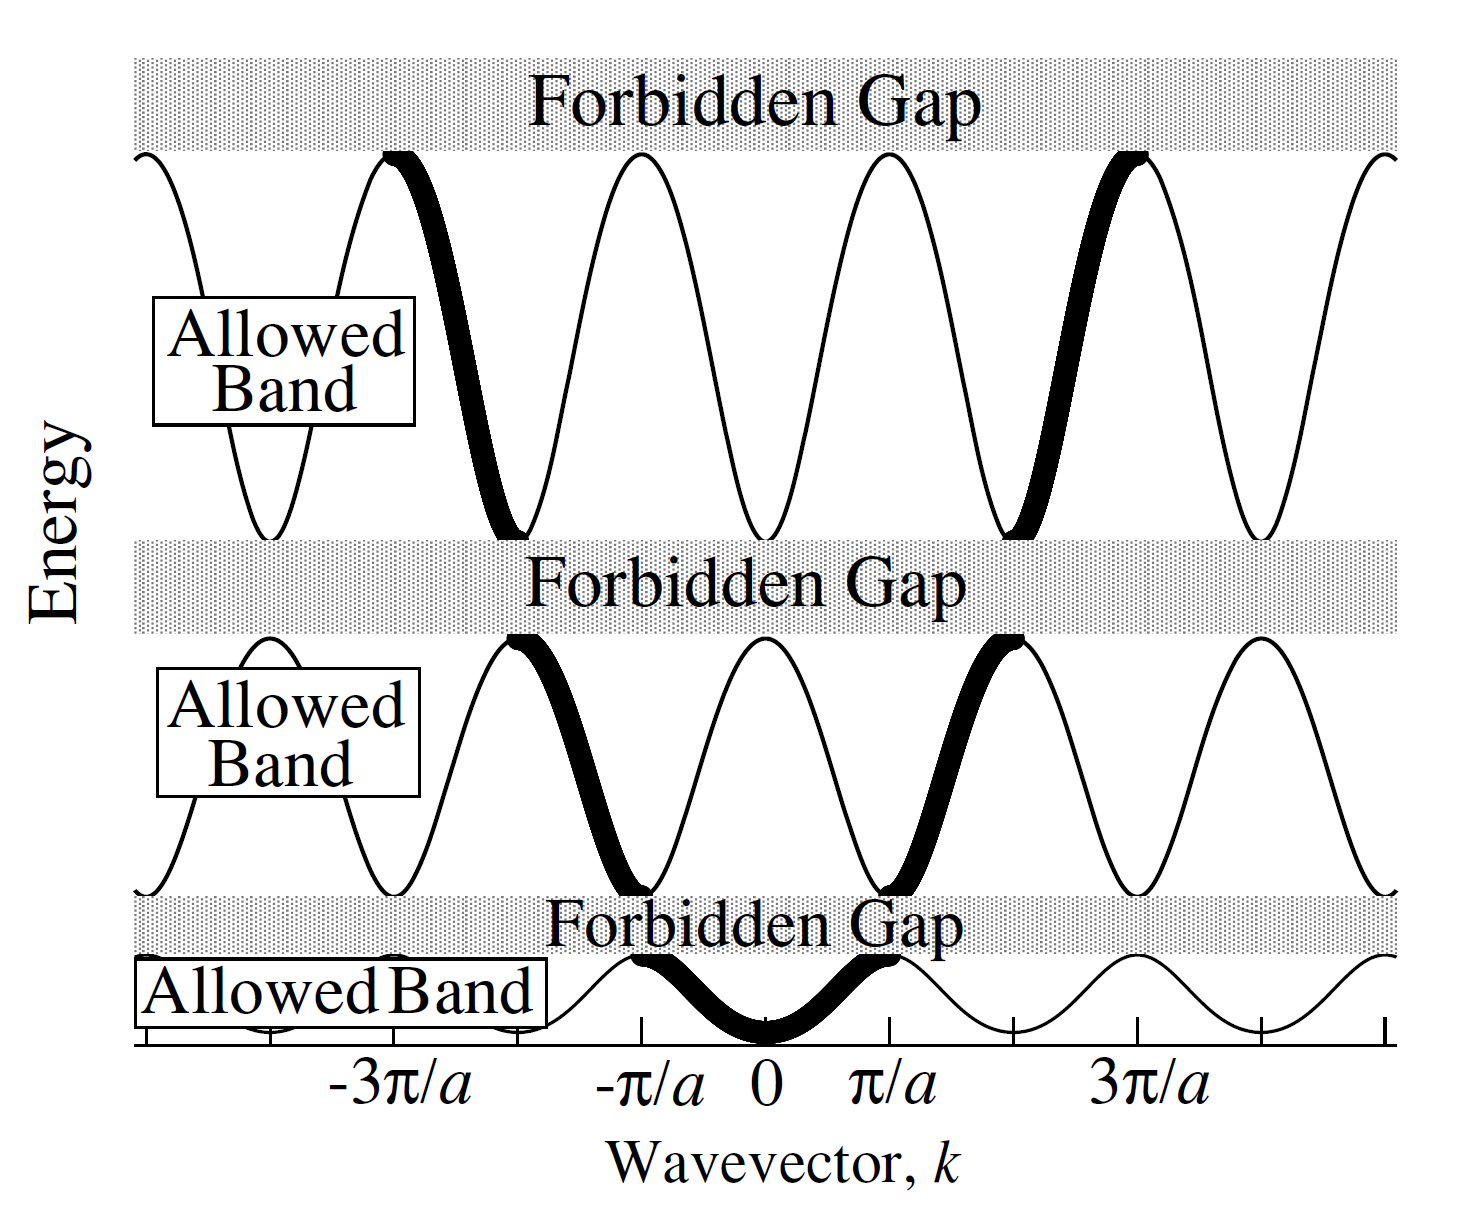
\includegraphics[scale=0.29]{Cuerpo/Ch_07/Oxford-03.png}
\caption{Dispersión en la aproximación de red vacía en el esquema extendido.}
\label{Fig:07-03a}
\end{subfigure} 
\begin{subfigure}{0.45\linewidth} \centering
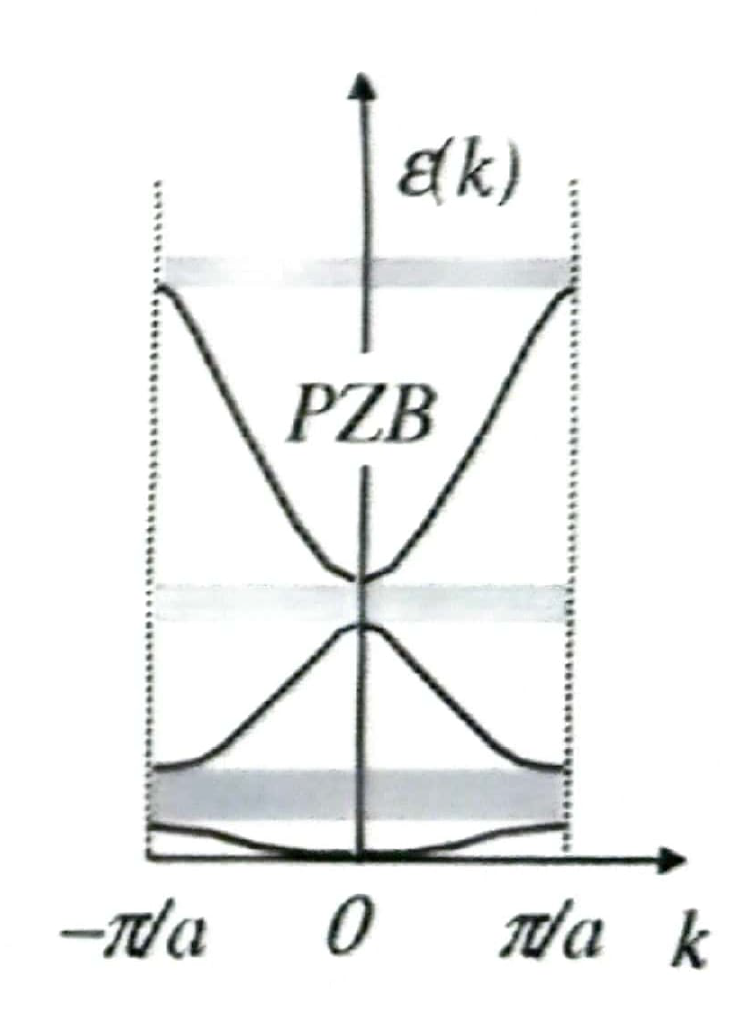
\includegraphics[scale=0.4]{Cuerpo/Ch_07/04.png}
\caption{Dispersión en la aproximación de red vacía en el esquema reducido.}
\label{Fig:07-03b}
\end{subfigure} 
\caption{Dispersión de la energía en función del momento en el esquema ampliado y reducido.}
\end{figure}   

Usando el concepto de la \textit{masa efectiva}, que es como recordamos la masa \textit{que tendría que tener nuestra carga} para que se comportará como un electrón libre, tenemos que los autovalores de la energía las podemos poner (aproximadamente):

\begin{eqnarray}
	E_+ (G+\delta) & = & C_+ + \frac{\hbar^2 \delta^2}{2m_+^*} \\
	E_- (G+\delta) & = & C_- - \frac{\hbar^2 \delta^2}{2m_+^*} 
\end{eqnarray}
donde la masa efectiva debe venir dada por

\begin{equation}
	m_{\pm}^* = \frac{m}{\left|1 \pm \frac{\hbar^2 (n\pi/a)^2}{m} \frac{1}{|V_G|} \right| }
\end{equation}


\subsection{Aproximación a red vacía en 2 y 3 dimensiones}

Los principios de la la aproximación a red vacía son muy similares en 2 y 3 dimensiones a los mencionados anteriormente: cerca de la zona de brillouin tenemos que aparece un gap debido a la interacción con un vector de onda separado por un vector  de la red recíproca. Esto generará dos estados, uno con más energía y otro con menos energía. Como podemos ver la generalización no es muy complicada, solo que ahora existirá que hay varios posibles $\kn'$ generados por la traslación de un vector de la red recíproca, por lo que la degneración es múltiple, y la matriz hamiltoniana a diagonalizar tendrá una extensión mayor. Este caso de varios estados con la misma energía lo podemos ver claramente en el caso 2 dimensional de la figura \ref{Fig:07-04}.

\begin{figure}[h!] \centering
	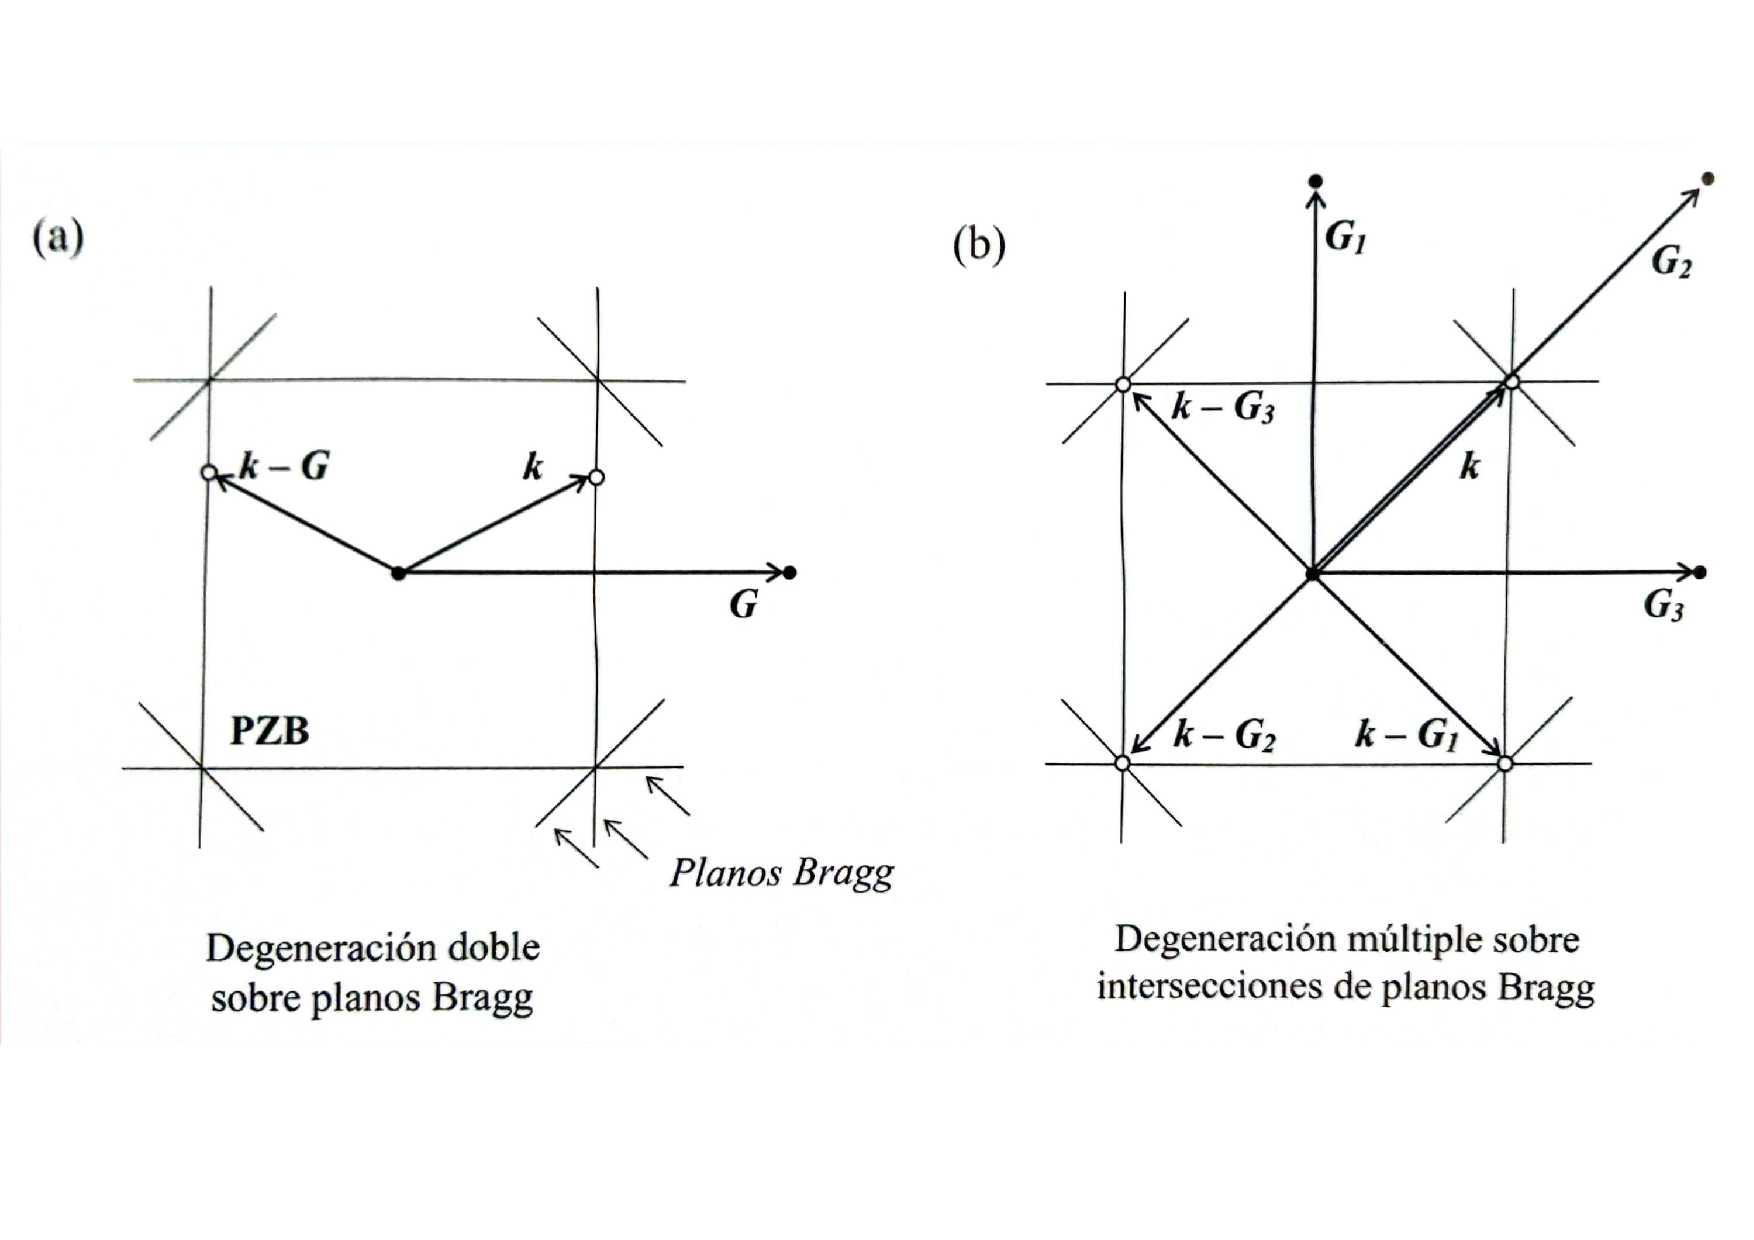
\includegraphics[scale=0.35]{Cuerpo/Ch_07/Fotos libro 2.pdf}
	\caption{(a) Ejemplo de estados doblemente degenerados sobre planos Bragg de una red cuadrada. (b) Estados cuádruplemente degenerados sobre las esquinas de la PZB de una red cuadrada.}
	\label{Fig:07-04}
\end{figure}    

\section{Teorema de Bloch}

En el modelo de casi electrones libres o aproximación a red vacía partimos de que las ondas planas son perturbadas débilmente por un potencial periódico. Pero en los materiales reales, la interacción entre átomos/electrones puede ser tan fuerte que la teoría de perturbaciones no sea válida. ¿Cómo hacemos entonces para describir el comportamiento de los electrones sin ondas planas? El hecho es que, en realidad, el momento $\kn$ usando en las ondas planas no es una cantidad conservada, mientras que el momento del cristal si lo es. No importa como de fuerte sea el potencial periódico, el momento cristalino es conservado. Este hecho descubierto por Felix Bloch se convirtió en el \textbf{teorema de Bloch}:

\begin{mybox}
	El \textbf{teorema de Bloch} nos dice que un electrón en un potencial periódico se puede describir en términos de las autofunciones de la fomra
	
	\begin{equation}
		\Psi_\kn^\alpha (\rn) = e^{i\kn \cdot \rn} u_\kn^\alpha (\rn)
	\end{equation}
	donde $u_\kn^\alpha$ es un potencial periódico en la celda unitaria y $\kn$ es el momento cristalino que podemos escogerlo de tal forma que caiga en la primera zona de Brilluoin.
\end{mybox}
En el esquema de zona reducida existirán varios estados posibles con el mismo $\kn$ cada uno denotado por $\alpha$. La función periódica $u$ es usualmente llamada la \textbf{función de Bloch} y $\Psi$ la \textbf{función de odna plana modificada}. Como $u$ es periódico, tenemos que se puede expresar como la suma de ondas planas sobre la red recíproca:

\begin{equation}
	u_\kn^\alpha (\rn) = \sum_{\Gn} \tilde{u}^{\alpha}_{\Gn,\kn} e^{i\Gn \cdot \rn}
\end{equation}
Esto garantiza que $u_\kn^\alpha (\rn) = u_\kn^{\alpha} (\rn + \Rn)$ para cualquier \textit{vector de red}. Esta es otra manera de expresar el teorema de Bloch, de tal manera que la suma de ondas planas $\kn$ pueden diferir por un conjunto de vectores recíprocos $\Gn$.

Una de las consecuencias del teorema de Bloch es que aquellas ondas que no estén separadas por un vector de ondas de la red recíproca no son capaces de interaccionar, esto es, que $\langle \kn'|V|\kn \rangle=0$ si $\kn' \neq \kn + \Gn$, de lo cual se deduce que en realidad la ecuación de Schrödinger 

\begin{equation}
	\ccorchetes{\frac{\pn^2}{2m} + V(\rn)} \Psi (\rn) = E \Psi (\rn)
\end{equation}
en el espacio de momentos 


\begin{equation}
	\sum_{\Gn} V_{\Gn} \Psi_{\kn - \Gn} =\ccorchetes{E-\frac{\pn^2}{2m}}\Psi_{\kn }
\end{equation}
donde $V_{\kn-\kn'}$ no es cero si $\kn-\kn'=\Gn$. Entonces es claro que tenemos una ecuación de Schrödinger para un conjunto de $\Psi_{\kn-\Gn}$ que verifique que $\Psi_\kn^\alpha (\rn) = e^{i\kn \cdot \rn} u_\kn^\alpha (\rn)$.

Aunque debe no debería ser sorprendendente que los electrones en un potencial periódico se comporten como una combinación lineal de ondas planas en función del momento cristalino, no debemos subestimar la importancia del teorema de Bloch. Este teorema nos dice que incluso cuando el potencial del electrón siente cada átomo de manera muy fuerte, los electrones siguen comportándose como si no sintieran a los átomos, siendo casi electrones libres. 



\section{Electrones fuertemente ligados}

En esta sección vamos a aproximar el cálculo de las funciones de onda y energías electrónicas en el caso de que que los átomos próximos perturben levemente los estados atómicos, enfoque particularmente útil para describir electrones de bandas internas $d$ de metales de transición y aislantes.  

Consideramos para simplificar una cristal monoatómico, y denotamos por $\epsilon_n$, $\phi_n$ las energías y autoestados atómicos: $\Hcal_{\text{at}} \phi_n = \epsilon_n \phi_n$. La aproximación lineal es probar como solución $\Psi_\kn (\rn) = \sum_\Rn C_\kn \Phi  (\rn - \Rn)$, donde la función $\Phi$ será una combinación lineal de orbitales atómicos degenerados $\Phi (\rn) = \sum_n b_n \phi_n (\rn)$. Debemos exigir que $\Psi_\kn$ sea de la forma de Bloch. Esto se cumple si $C_\kn (\Rn) = e^{i \kn \cdot \Rn}$, como es fácil de comprobar, con lo que 

\begin{equation}
	\Psi_\kn (\rn) = \sum_\Rn e^{i \kn \cdot \Rn} \Psi (\rn - \Rn) \label{Ec:07-05-01}
\end{equation} 
Por otro lado el hamiltoniano completo será 

\begin{equation}
	\Hcal = \Hcal_{\text{at}} + \Delta U(\rn)
\end{equation} 
donde $\Delta U (\rn)$ se supone sólo apreciable lejos de los iones (figura \ref{Fig:07-05}).

\begin{figure}[h!] \centering
	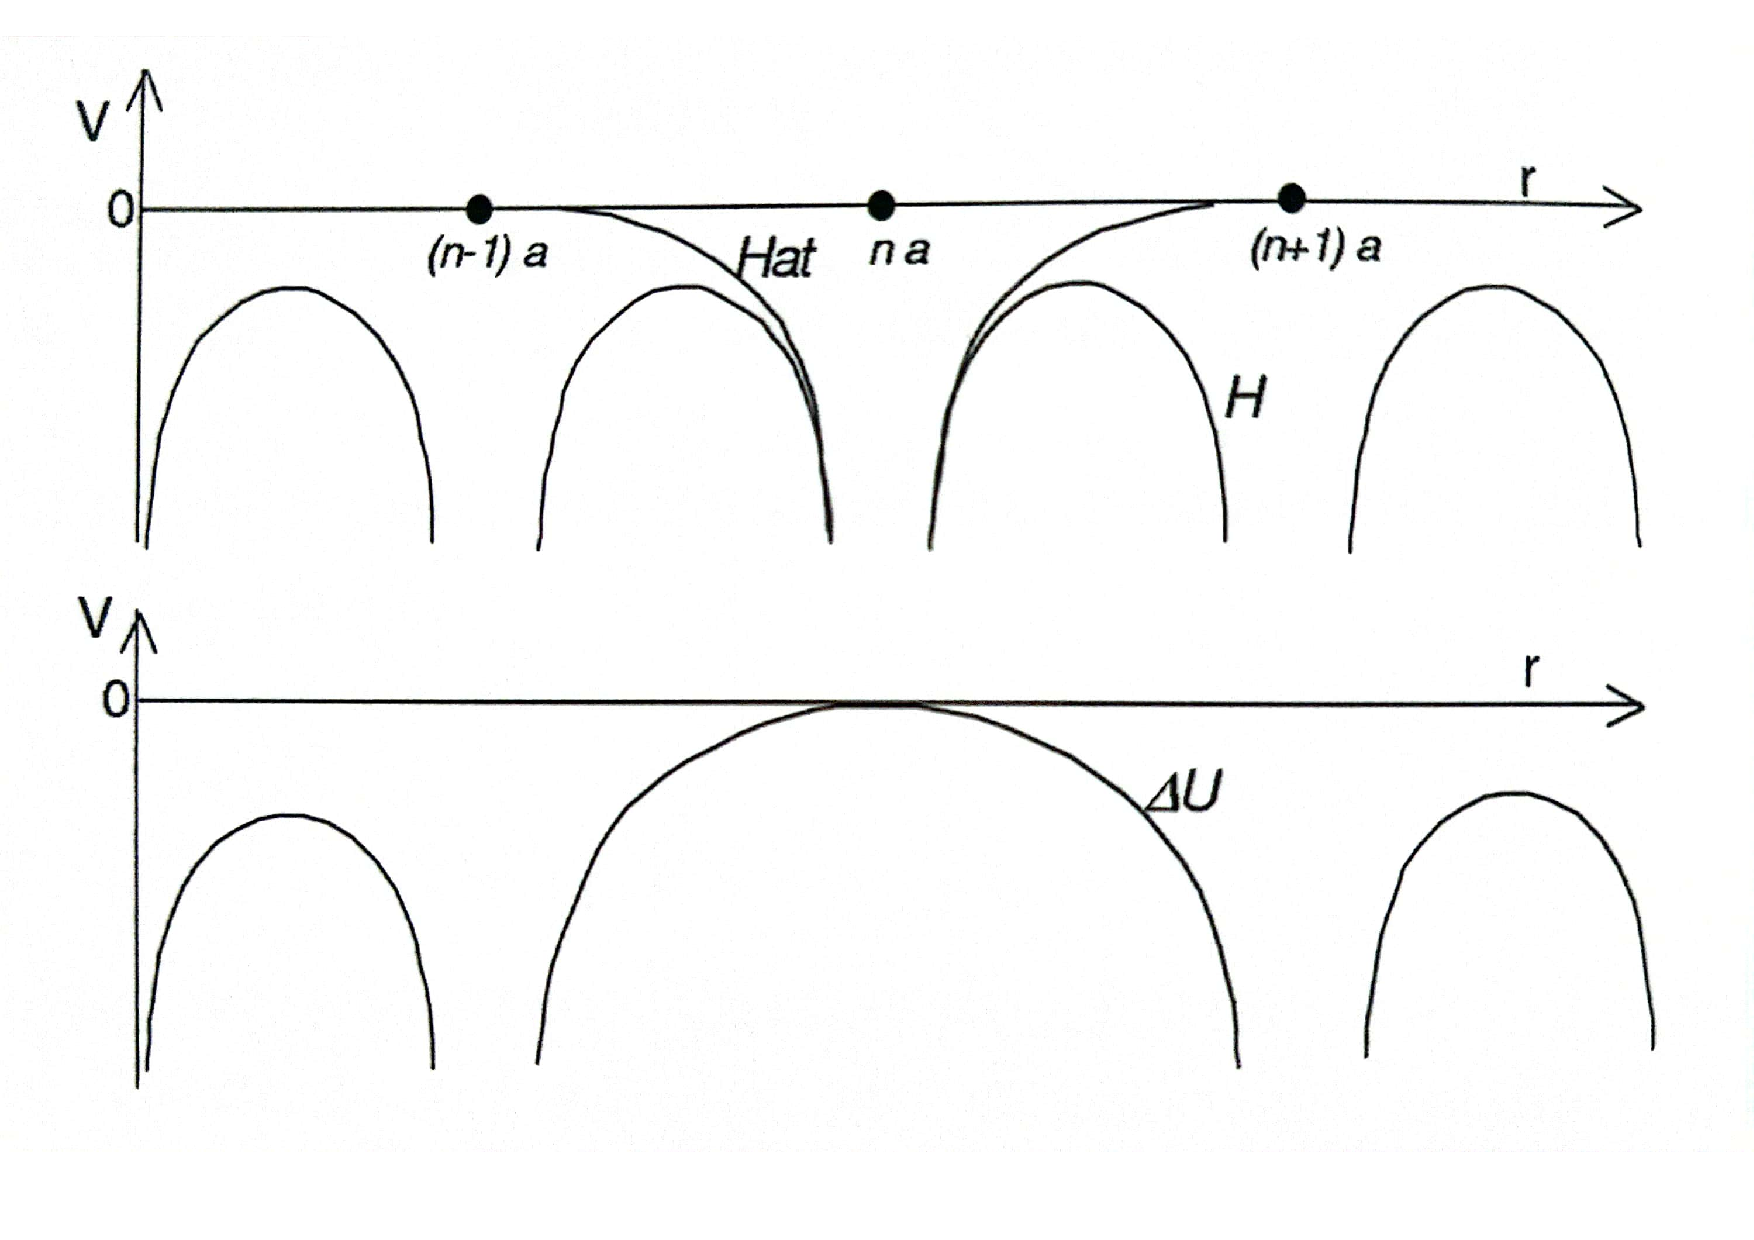
\includegraphics[scale=0.3]{Cuerpo/Ch_07/Fotos libro 5.pdf}
	\caption{Potencial periódico expresado como suma de un potencial atómico más una perturbación.}
	\label{Fig:07-05}
\end{figure}    
Utilizando la ecuación se Schrödinger podemos hallar que

\begin{equation}
	(\Hcal_\text{at} + \Delta U) |\Psi_\kn \rangle = \varepsilon(\kn) |\Psi_\kn \rangle
\end{equation}
que multiplicando por $\langle \psi_s |$   

\begin{equation}
	\varepsilon_s \langle \phi_s |\Psi_\kn \rangle + \langle \phi_s | \Delta U |\Psi_\kn \rangle = \varepsilon(\kn) \langle \phi_s |\Psi_\kn \rangle
\end{equation}
y despejando 

\begin{equation}
	\varepsilon(\kn) = \varepsilon_s + \frac{\langle \phi_s |\Delta U | \Psi_\kn \rangle}{\langle \phi_s |\Psi_\kn \rangle}
\end{equation}
utilizando ahora la ecuación (\ref{Ec:07-05-01}) e introduciendo la simplificación de considerar en $\phi$ sólo orbitales de tipo $s$:

\begin{equation}
	\begin{split}
		\varepsilon (\kn) \ = \ & \ \varepsilon_s  + \frac{\sum_\Rn e^{i \kn \cdot \Rn }\int \phi_s (\rn) \Delta U (\rn) \phi_s (\rn - \Rn) \D^3 \rn }{\sum_\Rn e^{i \kn \cdot \Rn }\int \phi_s (\rn)\phi_s (\rn - \Rn) \D^3 \rn }\\
		& \varepsilon_s -  \frac{\beta + \sum_{\Rn\neq 0} \gamma(\Rn) e^{i\kn \cdot \Rn}}{1+\sum_{\Rn\neq 0} \alpha (\Rn) e^{i\kn \cdot \Rn}}
	\end{split}
\end{equation}
donde hemos usado la siguiente notación: 

\begin{equation}
	\begin{split}
		\beta \ = \ &  \ - \int   \D^3 \rn \Delta U (\rn) |\phi_s (\rn) |^2 \\
		\alpha (\Rn) \ = \ & \ \int \D^3\rn \phi_s^* (\rn) \phi_s (\rn-\Rn) \\
		\gamma (\Rn) \ = \ & - \int \D^3 \rn \phi_s^* (\rn) \Delta U (\rn) \phi_s (\rn - \Rn)
	\end{split}
\end{equation}
Teniendo en cuenta que para un nivel s $\Psi (\rn) = \Psi (r)$, y que para un cristal monoatómico existe simetría de inversión ($\Rn \rightarrow - \Rn$) se tiene $\gamma (\Rn) = \gamma (R)$, $\alpha (\Rn) = \alpha (R)$ y $e^{i \kn \cdot \Rn} = \cos (\kn \cdot \Rn)$. Finalmente, despreciando $\gamma$ y $\alpha$ salvo para los vecinos más próximos (vmp), resulta:

\begin{equation}
	\varepsilon(\kn) = \varepsilon_s - \frac{\beta + \gamma_{\text{vmp}} \sum_{\text{vmp}} \cos (\kn \cdot \Rn)}{1+\alpha_{\text{vmp}} \sum_{\text{vmp}} \cos (\kn \cdot \Rn)}
\end{equation}
En ocasiones, puede también despreciarse la pequeña contribución de $\alpha_{\text{vmp}}$ en el denominador, quedando

\begin{equation}
	\varepsilon(\kn) = \varepsilon_s - \beta - \gamma_{\text{vmp}} \sum_{\text{vmp}} \cos (\kn\cdot \Rn)
\end{equation}
El resultado es que cada nivel atómico discreto da lugar a una banda posible de valores de la energía (dependientes de $\kn$), cuya anchura está controlada por $\gamma$. Es importante que este modelo puede dar lugar a \textit{solapamiento} entre bandas (que para cierto $\kn$ una banda tenga mayores valores de $\varepsilon$ que la banda inmediatamente superior) incluso en 1D (figura \ref{Fig:07-06}). 


\begin{figure}[h!] \centering
	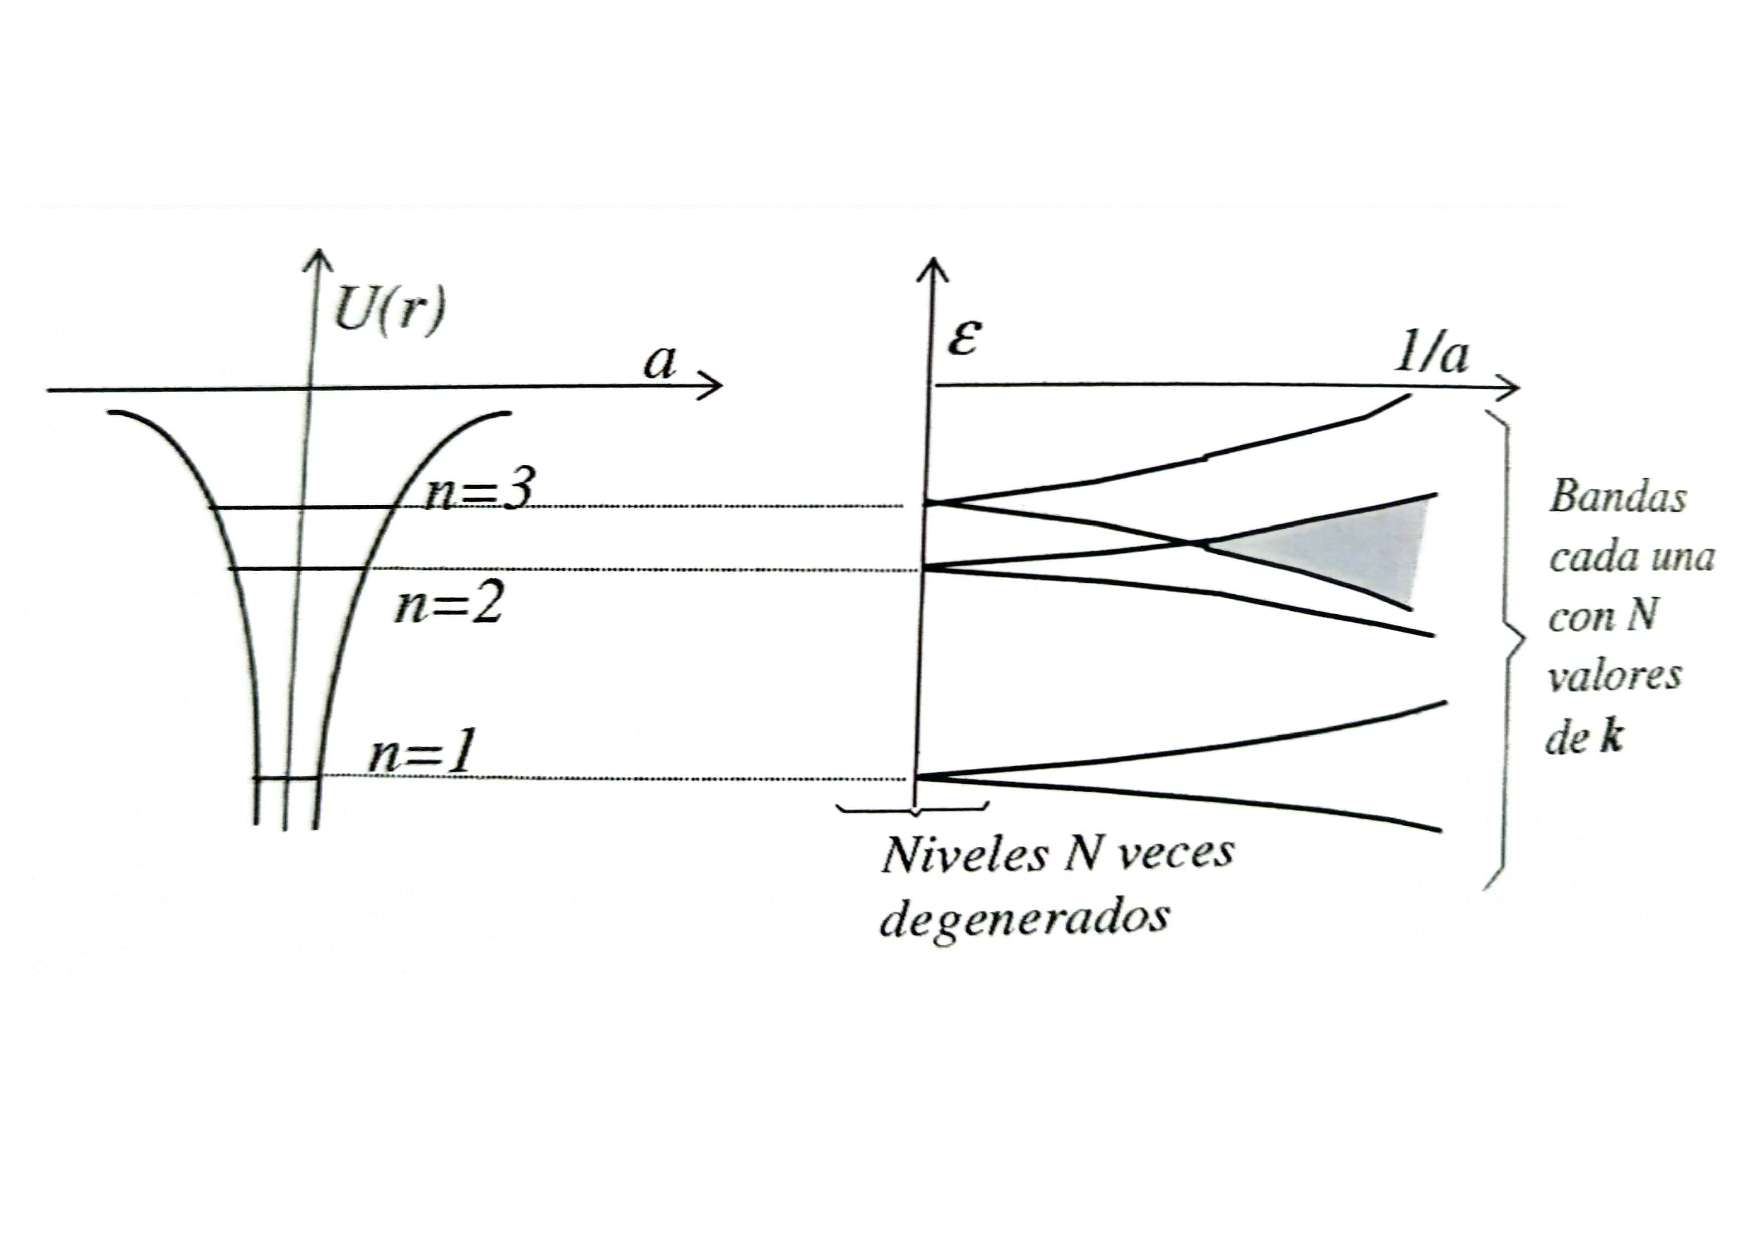
\includegraphics[scale=0.35]{Cuerpo/Ch_07/Fotos libro 6.pdf}
	\caption{Bandas de energía a partir de la aproximación de electrones fuertemente ligados. La zona sombreada representa el solapamiento entre la 1ª y 2ª bandas.}
	\label{Fig:07-06}
\end{figure}    

\section{Superficie de Fermi y zonas de Briollouin}

Una vez conocida la relación de dispersión monoeléctria $\varepsilon(\kn)$, se estudia a continuación como se ocupan los distintos niveles energéticos con los electrones aportados por el cristal. El concepto de la superficie de Fermi (estudiada en el capítulo anterior) como la superficie en el espacio de fases que separa, a $T=0$ K, los estados electrónicos llenos de los vacío, sigue teniendo sentido. Como se verá, la relación topológica entre la superficie de Fermi y las zonas de Brillouin es determinante para muchas propiedades metálicas.

\begin{figure}[h!] \centering
	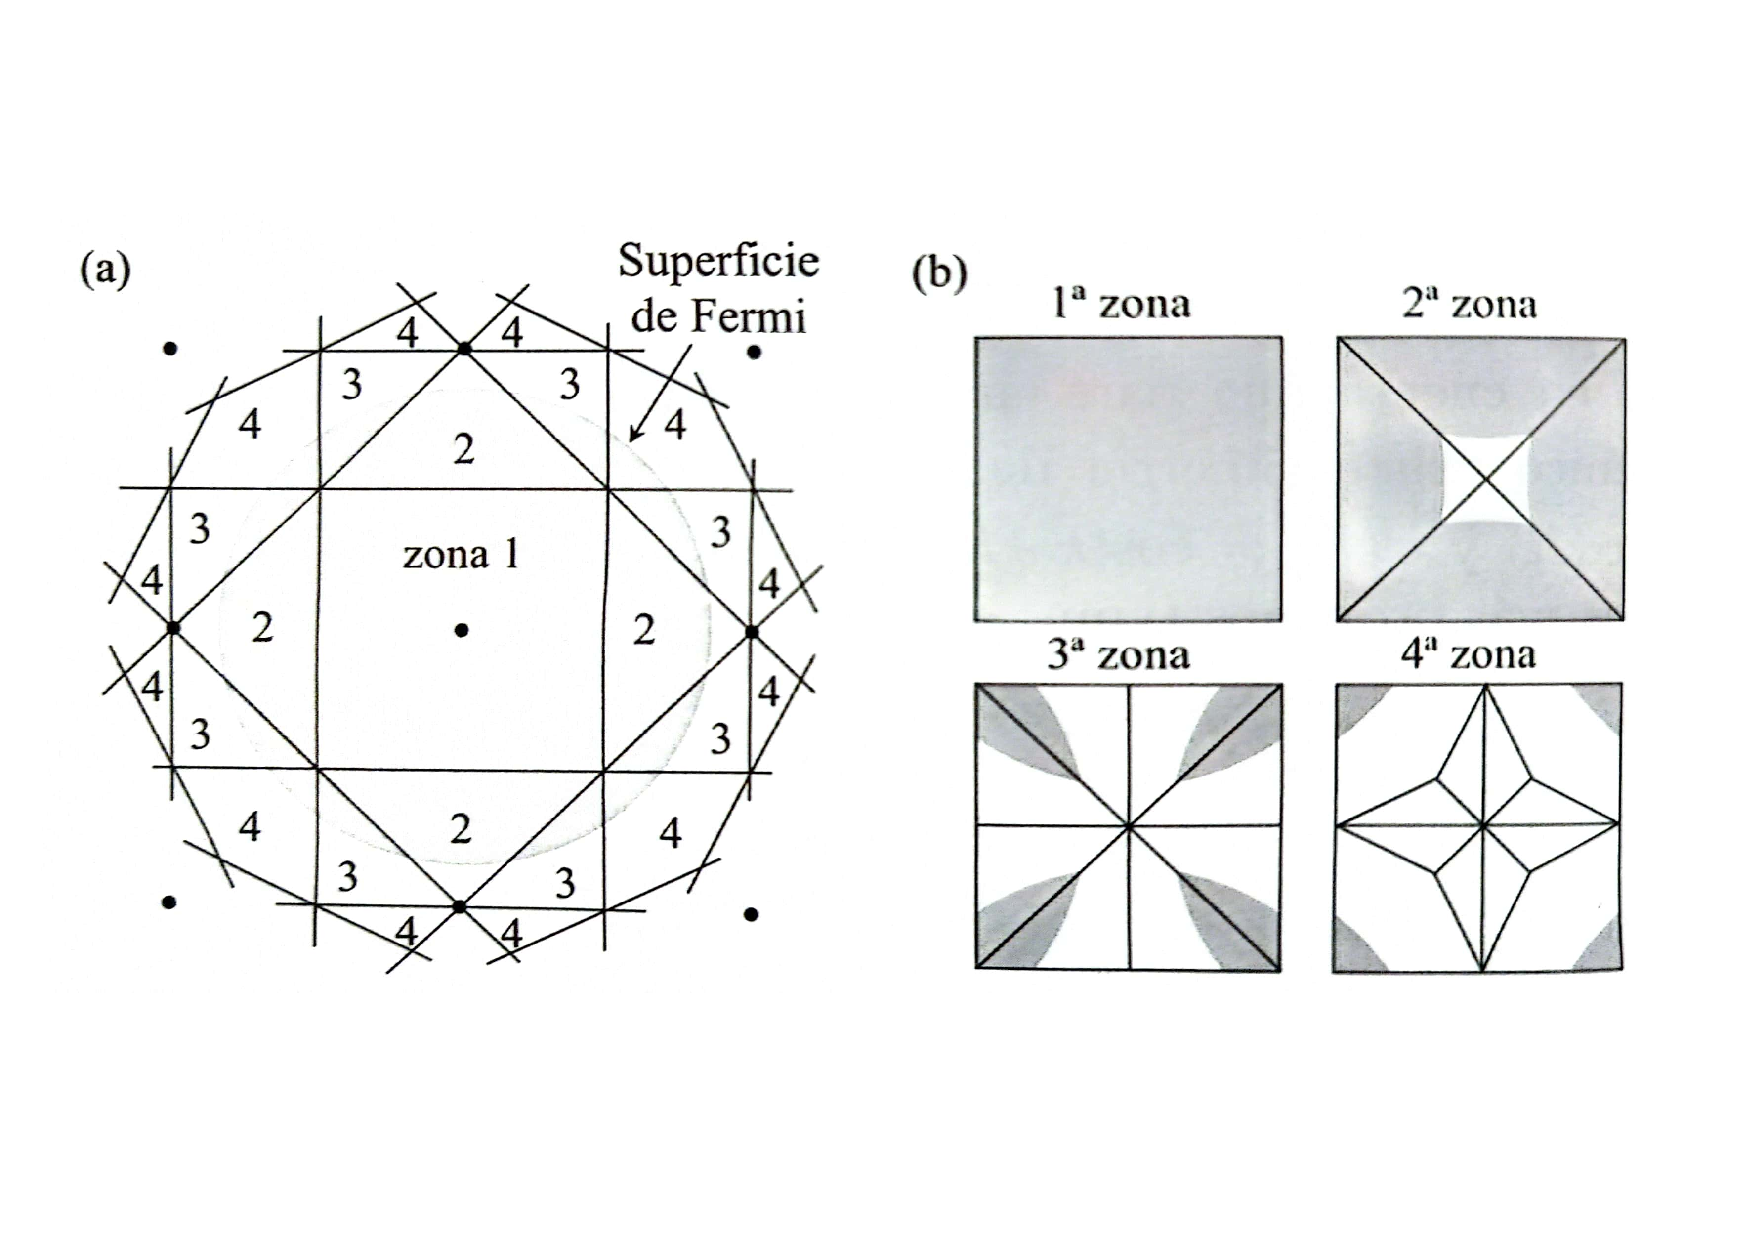
\includegraphics[scale=0.35]{Cuerpo/Ch_07/Fotos libro 7.pdf}
	\caption{1ª, 2ª, 3ª y 4ª zonas de Brillouin para una red cuadrada 2D, según los esquemas en zona extendida (a) y reducida (b). En gris se representan los estados ocupados.}
	\label{Fig:07-07}
\end{figure}    

En la figura \ref{Fig:07-07} (a) se encuentran las primeras zonas de Brillouin para la red cuadrada, y la superficie de Fermi en la aproximación de red vacía. En este ejemplo, la primera zona de Brillouin (PZB) está completamente llena, y la 2ª (SZB), 3ª (TZB) y 4ª (CZB) parcialmente llenas. Se puede hacer una transformación al esquema en zona reducida por las traslaciones en vectores de red y resulta lo que ilustra la figura \ref{Fig:07-07} (b) (obsérvese que todas las zonas tienen el mismo volumen fásico). Las regiones grises son las ocupadas por electrones y tienen una energía inferior a la de las regiones blancas. En la figura \ref{Fig:07-08} se muestran otros ejemplos de zonas de Brillouin, esta vez para la estructuras \bcc y \fcc. Finalmente, en la figura \ref{Fig:07-09} se muestra un ejemplo, correspondiente a una estructura \fcc, de cómo es la relación topológica entre las zonas de Brillouin y la superficie de Fermi para electrones libres, según la valencia de los átomos que componen la estructura. 

La forma real de la superficie de Fermi puede determinarse mediante experimentos de magnetorresistencia, efecto pelicular anómalo, resonancia ciclotrón, magnetoacústica y el efecto Haas-van Alphen (oscilación del momento magnético de un metal en función de la intensidad del campo mangético aplicado). Como ya se explicó anteriormente, las superficies de Fermi se ven más deformadas (respecto de las de electrones libres) cerca de las fronteras de zona, de modo que en general las cortas perpendicularmente.

\begin{figure}[h!] \centering
	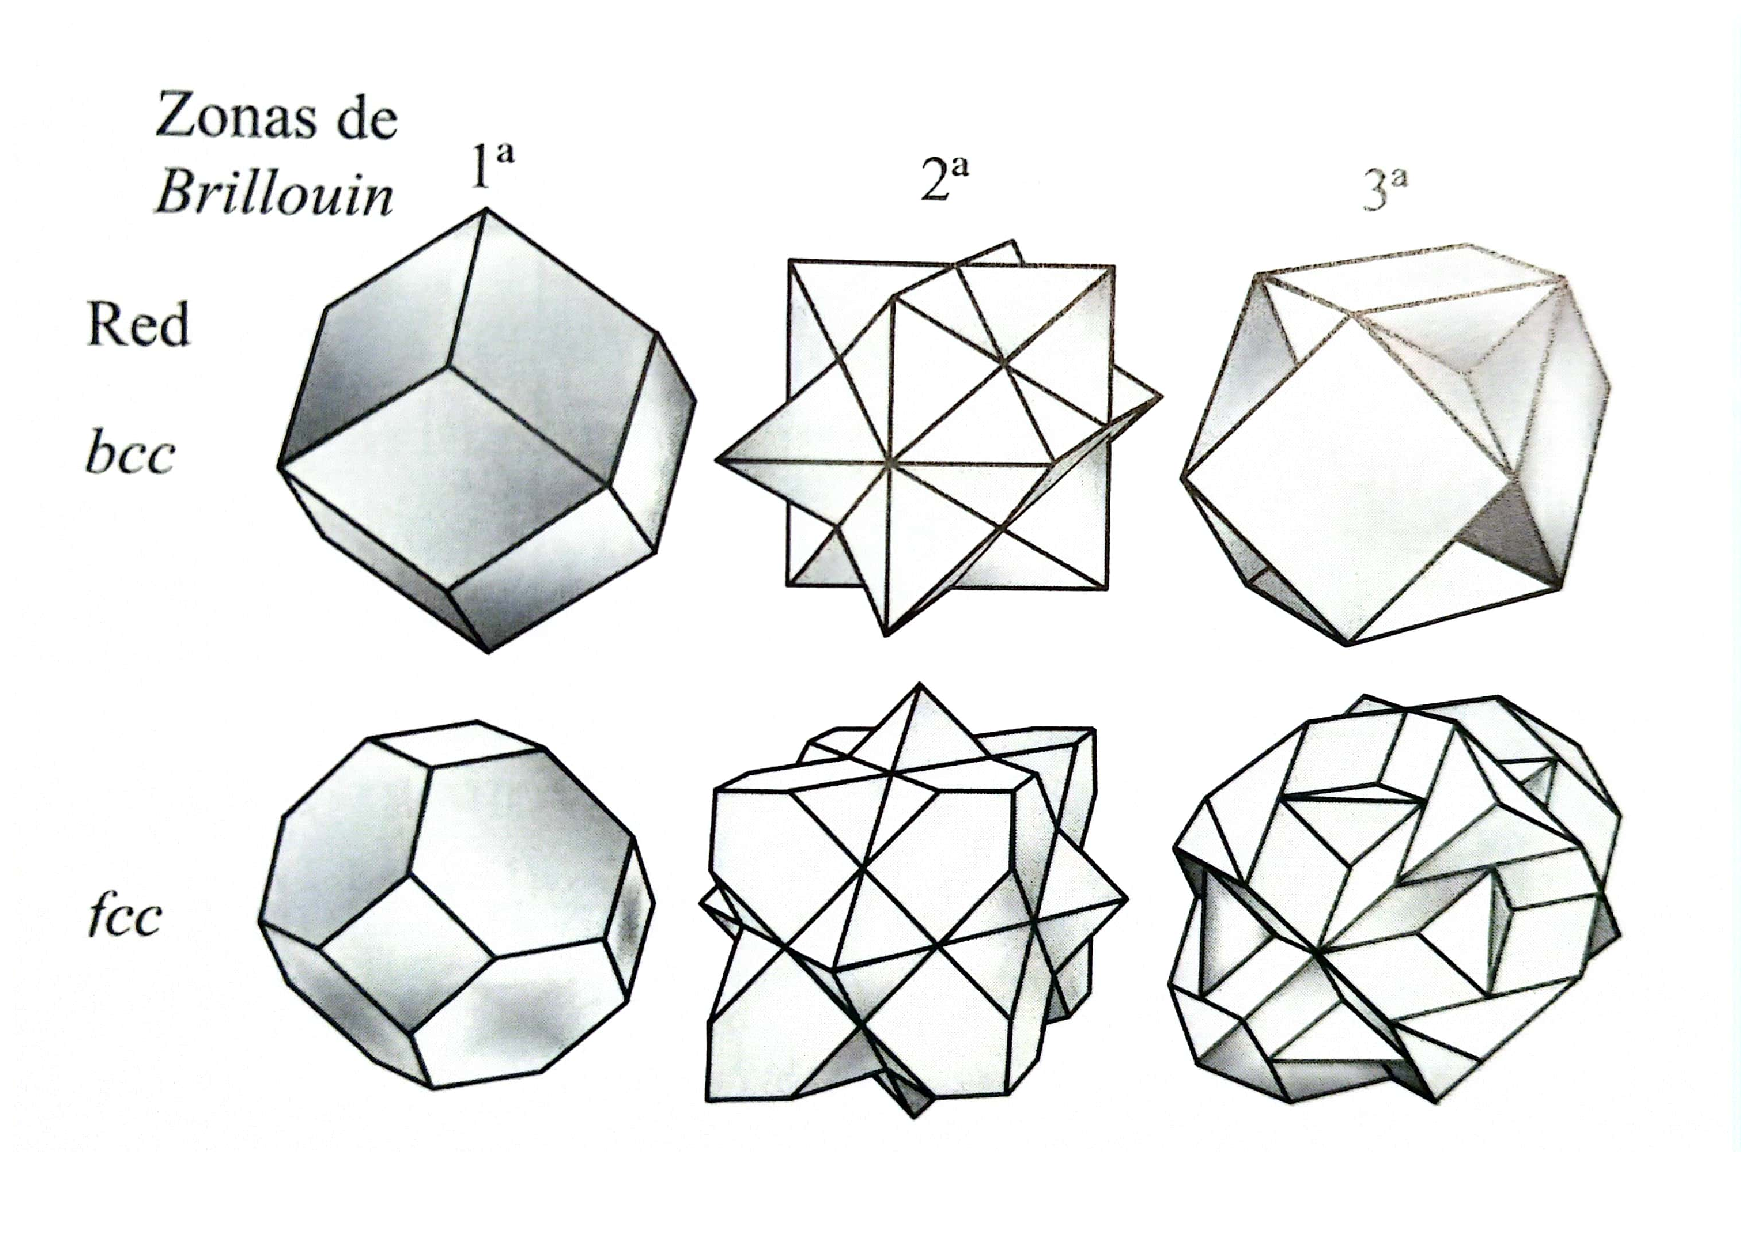
\includegraphics[scale=0.35]{Cuerpo/Ch_07/Fotos libro 8.pdf}
	\caption{Primeras zonas de Brillouin para las estructuras \bcc y \fcc, según el esquema en zona reducida.} 
	\label{Fig:07-08}
\end{figure}    
\begin{figure}[h!] \centering
	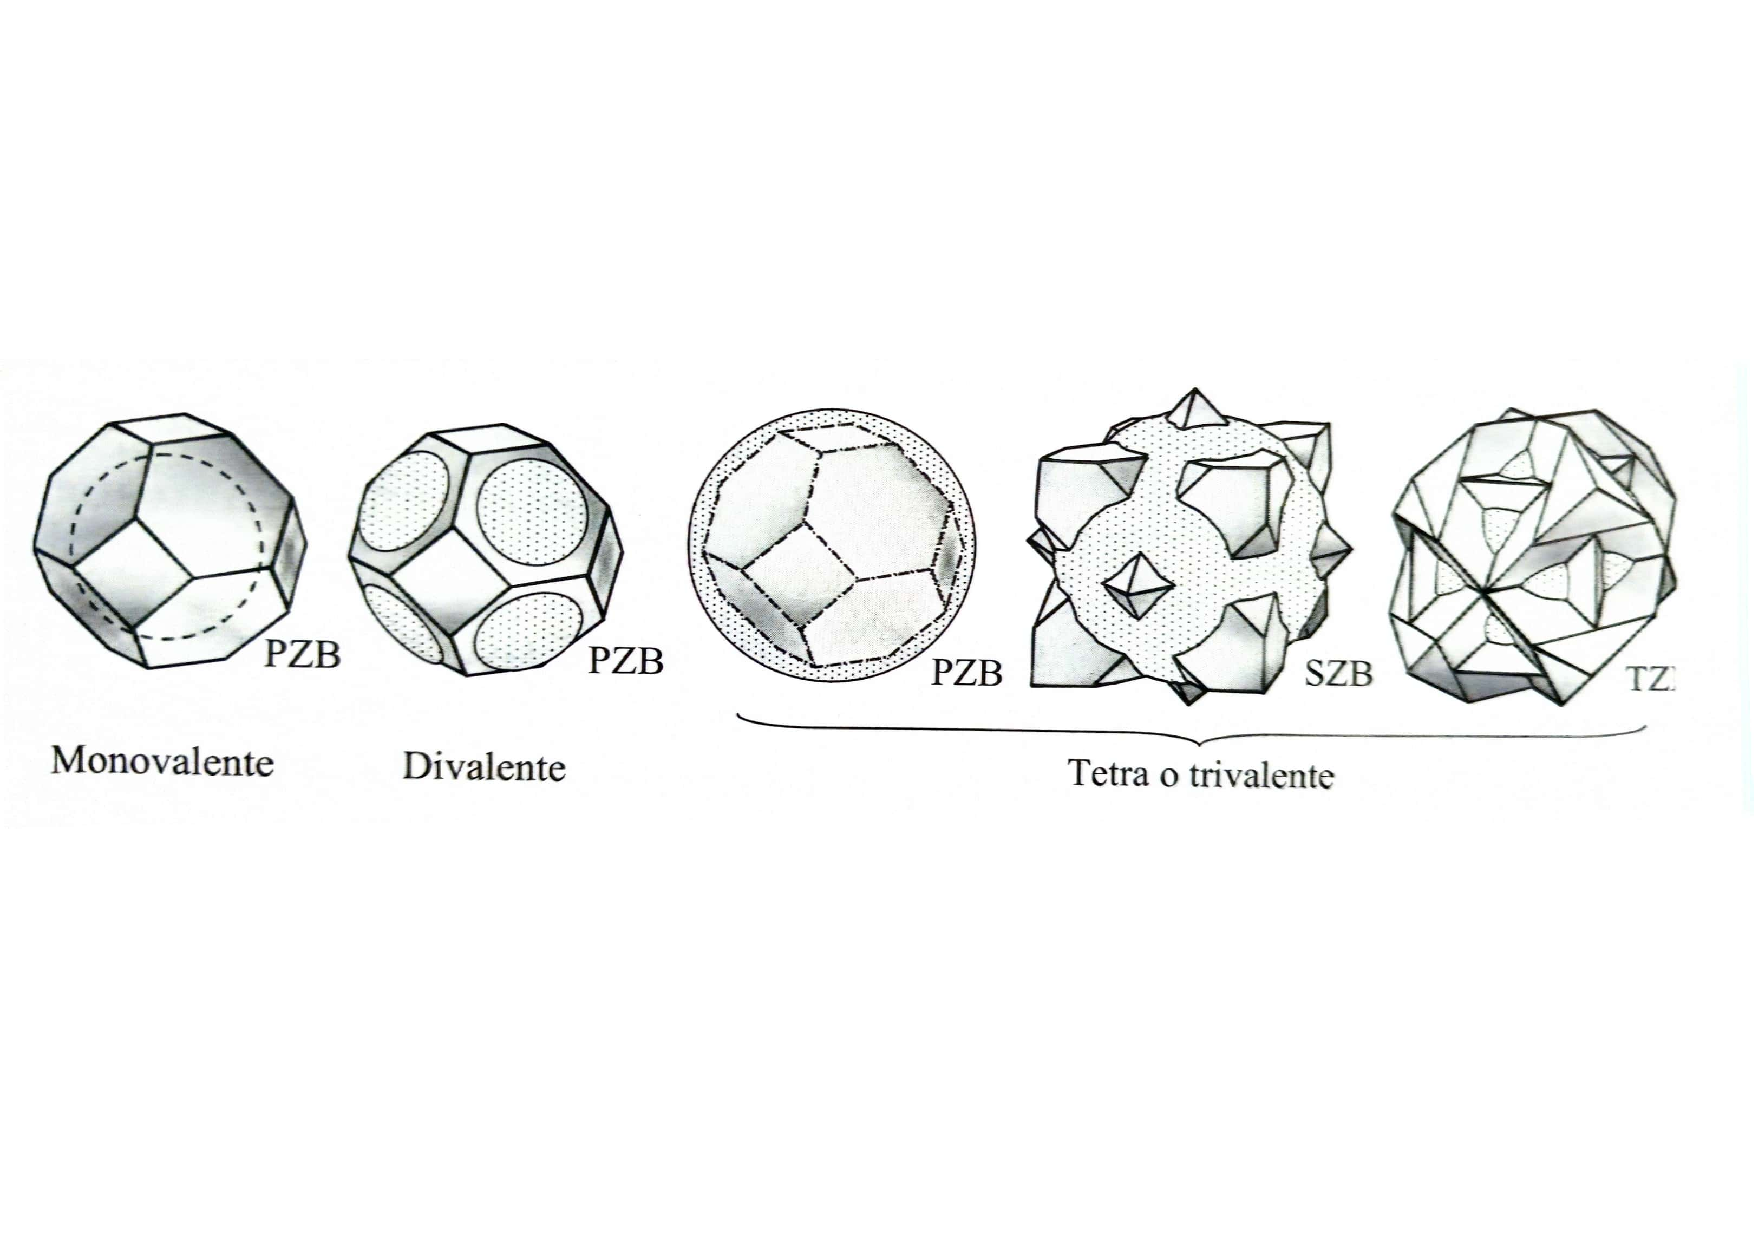
\includegraphics[scale=0.45]{Cuerpo/Ch_07/Fotos libro 9.pdf}
	\caption{Relación entre las primeras zonas de Brillouin de la estructura \fcc y la superficie de Fermi de electrones libres (esférica), según la valencia atómica.}
	\label{Fig:07-09}
\end{figure}    


\section{Metales, aislantes y semiconductores}

La importancia del ``mapeo'' de la superficie de Fermi en las distintas zonas, del que hemos visto algunos ejemplos, viene de lo siguiente. Como se verá en detalle en el siguiente Capítulo \ref{Ch:08}, debido al gap de energía en las fronteras de zona, las bandas llenan son aislantes, las zonas casi llenas conducen por cargas positivas, y las casi vacías por cargas negativas. Hay que recordar también que, como hemos visto, el número de electrones posibles en una zona o banda es $2N$ siendo $N$ el número de celdas primitivas en el cristal. En base a esto caben varias posibilidades: una sustancia con un número \textit{impar} de electrones de valencia por celda primitiva será siempre un \textit{metal} (conductor) ya que no puede llenar bandas enteras. Si el número de electrones es \textit{par} es necesario saber si las bandas sucesivas se solapan en energía o no. Si no hay solapamiento será \textit{aislante} y si solapan sucesivas (o \textit{semimetal} si el solapamiento pequeño). Podría darse también el caso de materiales aislantes con un gap de energía tan pequeña ($<1$ eV) que para $T\neq 0$ K conduzcan por promoción térmica de electrones entre bandas (\textit{semiconductores}). Estas posibilidades se esquematizan en la figura \ref{Fig:07-10}.

\begin{figure}[h!] \centering
	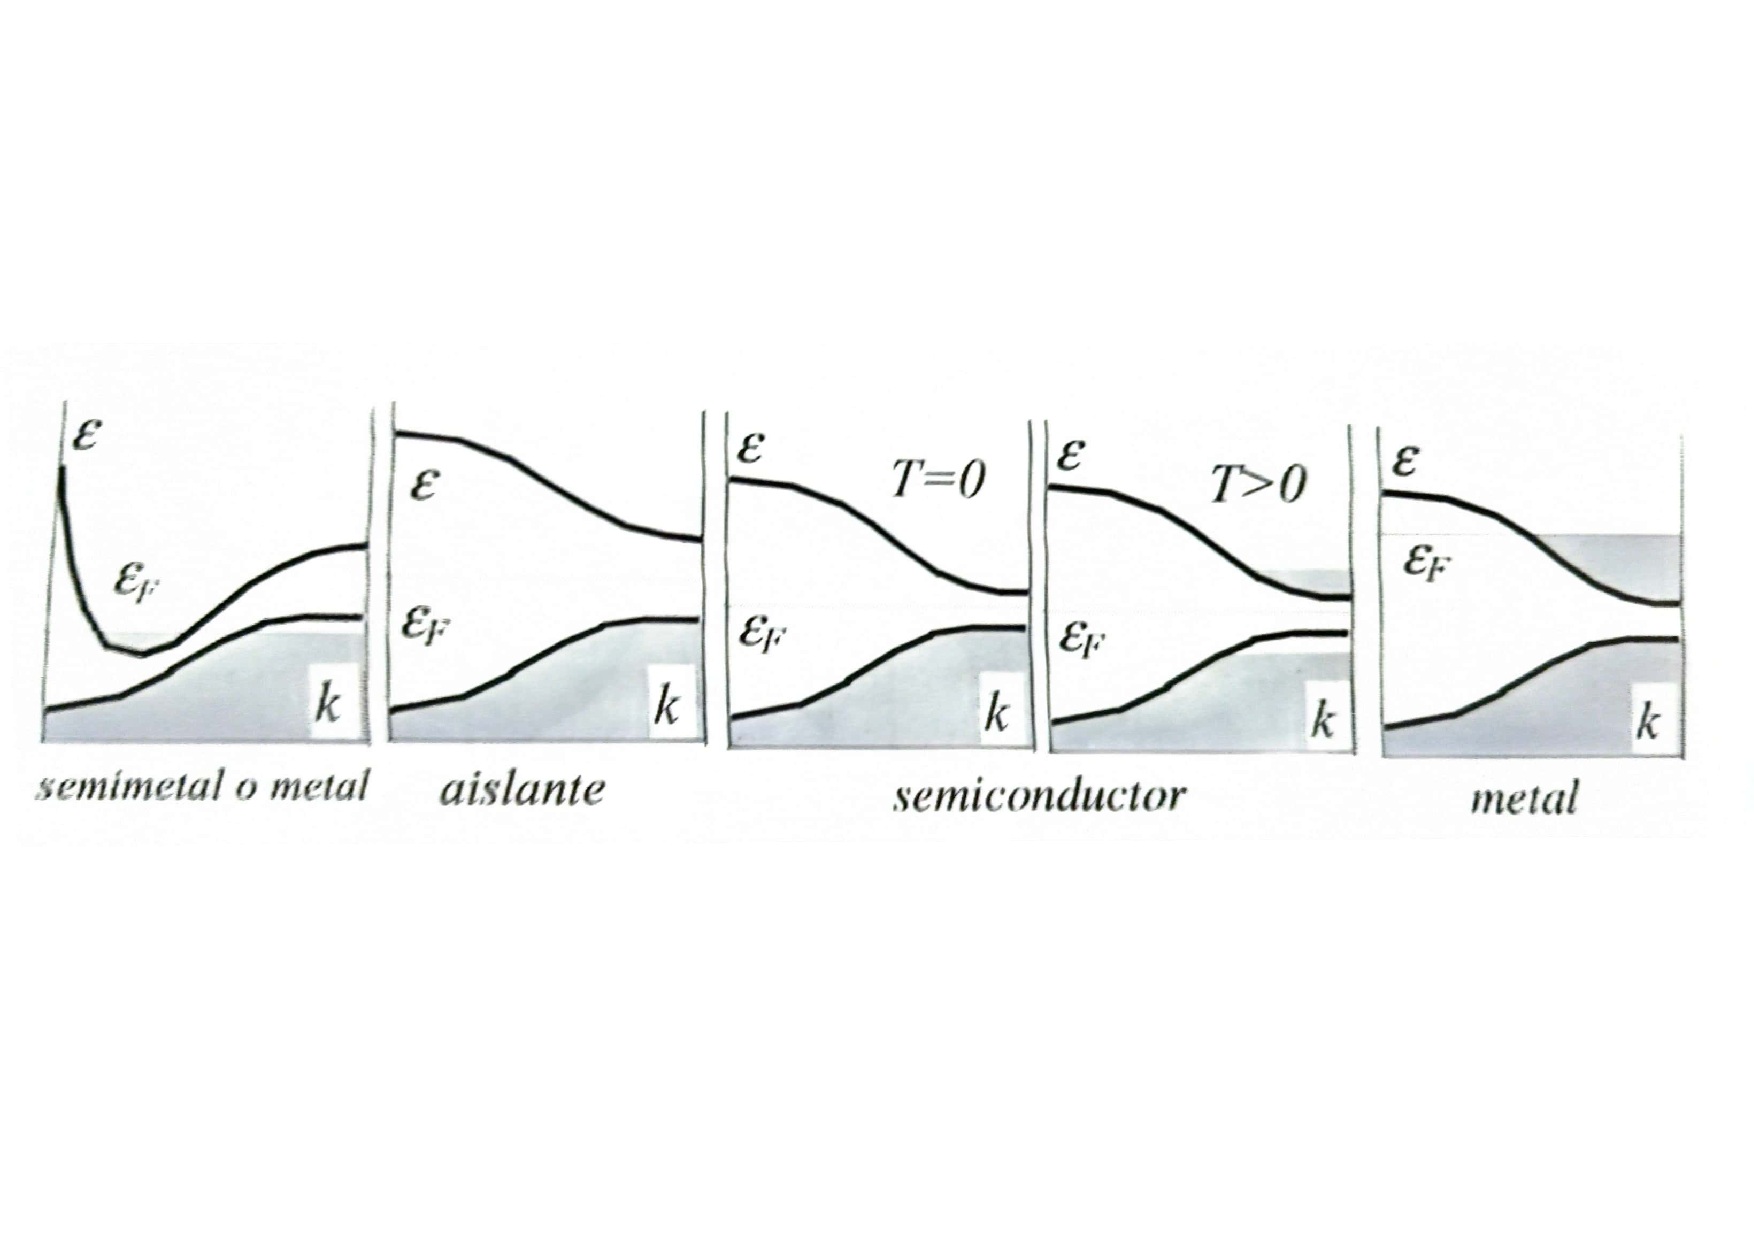
\includegraphics[scale=0.5]{Cuerpo/Ch_07/Fotos libro 10.pdf}
	\caption{Clasificación de los sólidos según la relación que hay entre el nivel de Fermi y la estructura de bandas.}
	\label{Fig:07-10}
\end{figure}    




